\documentclass{article}
\usepackage{graphicx}
\usepackage{standalone}
\usepackage{multicol}
\usepackage{amsmath}
\begin{document}
    \section{Task}
    \begin{minipage}{0.5\textwidth}
Consider the following continuous benchmark function SPHERE:
	
$\displaystyle SPHERE(x) = \sum_{i=1}^{n} x_i^2  \text{with}  -\infty < x < \infty$
\\

The SPHERE function has a unique global minimum in:

$\displaystyle SPHERE(x_1,\dotsc,x_n) = SPHERE(0,\dotsc,0) = 0$
\end{minipage}
\begin{minipage}{0.5\textwidth}
    \begin{flushright}
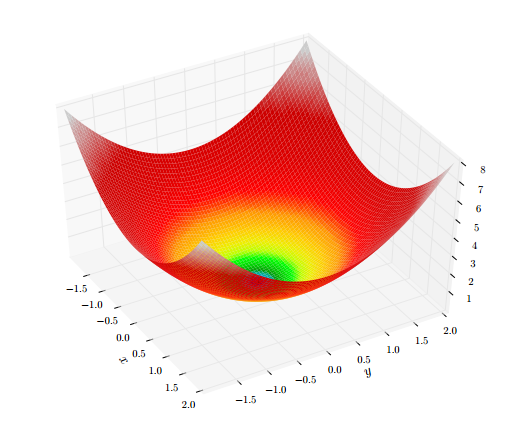
\includegraphics[width=\textwidth]{GraphOriginal}
\end{flushright}
\end{minipage}

and can be visualised for n = 2 as shown above. It is a suitable benchmark to investigate if and
how an algorithm starting from some arbitrary point in the search space is able to converge to a
local optimum, which is an important property for nature-inspired algorithms.
\\

In the lecture you have learned about two mutation operators in the context of continuous function
optimisation, uniform and non-uniform mutation. Here, we consider these and two additional
operators, Gaussian mutation with and without 1/5-rule. You can find explanations and pseudo code
for all four operators in the appendix of this assignment. Your task is to implement and compare
the performance of these four operators on the SPHERE function.
\end{document}